\documentclass[11pt,a4paper]{article}
\usepackage[utf8]{inputenc}
\usepackage[T1]{fontenc}
\usepackage{lmodern}
\usepackage[margin=2.2cm]{geometry}
\usepackage{amsmath,amssymb}
\usepackage{booktabs,array,tabularx,longtable}
\usepackage{graphicx}
\usepackage{xcolor}
\usepackage{enumitem}
\usepackage[most]{tcolorbox}
\usepackage[hidelinks]{hyperref}
\usepackage{microtype}
\graphicspath{{../paper/figures/}}

\definecolor{chim}{HTML}{2A78D6}
\definecolor{warn}{HTML}{B5560B}
\definecolor{good}{HTML}{147A50}
\newtcolorbox{idea}[1][]{colback=chim!6,colframe=chim!70,boxrule=0.6pt,arc=2pt,left=6pt,right=6pt,top=4pt,bottom=4pt,fonttitle=\bfseries,title={#1}}
\newtcolorbox{honest}[1][]{colback=warn!7,colframe=warn!75,boxrule=0.6pt,arc=2pt,left=6pt,right=6pt,top=4pt,bottom=4pt,fonttitle=\bfseries,title={#1}}
\newtcolorbox{viva}[1][]{colback=good!6,colframe=good!70,boxrule=0.6pt,arc=2pt,left=6pt,right=6pt,top=4pt,bottom=4pt,fonttitle=\bfseries,title={#1}}
\setlist{itemsep=2pt,topsep=3pt}
\setlength{\parskip}{4pt}
\setlength{\parindent}{0pt}
\newcommand{\Q}[1]{\par\medskip\textbf{Q. #1}\par}
\newcommand{\A}{\textit{Answer.}~}

\title{\textbf{CHIMERA, explained from zero}\\[4pt]
\large A complete guide to the project for people who have never seen it,\\
and preparation for a viva}
\author{Adithyan C S S \quad Ajay M \quad Rohith Pranov V\\[2pt]
\small Computer Science and Engineering, Vellore Institute of Technology, Vellore}
\date{October 2026}

\begin{document}
\maketitle

\begin{idea}[How to read this guide]
Part~1 (Sections 1--4) assumes nothing: it explains what the cloud, Kubernetes and
autoscaling are, and what problem the project solves. Part~2 (Sections 5--8) explains how
CHIMERA works and how it was tested. Part~3 (Sections 9--12) gives the results, including
where CHIMERA does \emph{not} win, and what went wrong along the way. Part~4 (Sections
13--16) is for the viva: the project map, a demo guide, about sixty questions with
answers, a glossary, and a one-page sheet of numbers to memorise.

If you have ten minutes, read Section~4 (the one-page summary) and Section~16 (the
numbers). If you have an hour, read everything.
\end{idea}

\tableofcontents
\newpage

%=====================================================================
\part*{Part 1 \quad The basics}
\addcontentsline{toc}{part}{Part 1: The basics}

\section{The world this project lives in}

\subsection{Applications run on servers, and servers cost money}
When you open an app, your phone sends a \emph{request} to a program running on a
computer in a data centre. That program does some work and sends a \emph{response}. The
computer's processor (CPU) is what does the work. CPU power is measured in
\textbf{cores}: one core can run one stream of work at a time. Companies rent cores from
cloud providers (Amazon, Google, Microsoft, Huawei, Alibaba) and pay for every core, for
every minute, whether it is busy or idle.

So there are two things a company wants at the same time:
\begin{enumerate}
\item \textbf{Fast responses.} Users leave if the app is slow.
\item \textbf{Low cost.} Every idle core is money thrown away.
\end{enumerate}
These pull in opposite directions. Many cores: fast but expensive. Few cores: cheap but
slow when traffic rises. Traffic also changes all the time: quiet at night, busy at noon,
and sometimes a sudden spike (a sale, a news event).

\subsection{Containers, pods and Kubernetes}
Modern applications are packaged as \textbf{containers}: a program plus everything it
needs, which runs the same way on any machine. \textbf{Kubernetes} is the most widely used
system for running containers on a group of machines (a \textbf{cluster}). In Kubernetes:
\begin{itemize}
\item A \textbf{pod} is one running copy of the application (one or more containers).
\item A \textbf{replica} is another identical copy of the pod. Ten replicas means ten
copies sharing the traffic.
\item Each pod has a \textbf{CPU limit}: the maximum CPU it may use, for example
\texttt{500m} (``500 millicores'', half a core) or \texttt{2} (two cores).
\end{itemize}

\subsection{Two ways to give an application more power}
\begin{center}
\begin{tabular}{@{}p{3.2cm}p{5.6cm}p{6cm}@{}}
\toprule
 & \textbf{Horizontal scaling} & \textbf{Vertical scaling} \\
\midrule
What changes & the number of pods (replicas) & the CPU of each pod \\
Analogy & open more checkout counters in a shop & make each cashier work faster \\
Speed & \textbf{slow}: a new pod must be scheduled, started and become ready, typically tens of seconds & \textbf{fast} since Kubernetes 1.33: about 0.1\,s, without restarting the pod (``in-place resize'') \\
Kubernetes tool & HPA (Horizontal Pod Autoscaler) & VPA (Vertical Pod Autoscaler) \\
\bottomrule
\end{tabular}
\end{center}

Until recently, changing a pod's CPU meant killing the pod and starting a new one, which
was slow and disruptive, so vertical scaling was rarely used for fast reactions.
\textbf{In-place pod resize} (Kubernetes Enhancement Proposal 1287, on by default from
Kubernetes 1.33 in 2025, stable in 1.35) changed this: the CPU of a running pod can now be
changed in a fraction of a second, without a restart. This is the key fact behind the
whole project.

\subsection{Autoscaling}
An \textbf{autoscaler} is a program that watches the application and changes its
resources automatically. The two standard ones in Kubernetes:
\begin{itemize}
\item \textbf{HPA} looks at average CPU utilisation. If it is above a target (say 70\,\%),
it adds pods; if below, it removes pods.
\item \textbf{VPA} looks at past CPU usage and sets a sensible CPU size for each pod.
\end{itemize}
Run together on the same signal, they can fight: the HPA adds pods, so each pod looks less
busy, so the VPA shrinks the pods, so each pod looks busy again, so the HPA adds pods\dots
And neither of them knows that a pod it just ordered is not serving yet.

\section{Words you must know}

\textbf{Latency (response time).} How long one request takes, in seconds.

\textbf{SLO (service level objective).} A promise about latency, for example ``every
request should finish within 0.5\,s''. A request that takes longer is an \textbf{SLO
violation}. The main quality number in this project is the \textbf{SLO violation rate}:
the percentage of requests that were too slow. Lower is better.

\textbf{p99 latency.} Sort all response times; the p99 is the value 99\,\% of requests
are faster than. It describes the slowest experiences (the ``tail'').

\textbf{Utilisation.} How busy the CPU is: demand divided by capacity. At 50\,\%
utilisation the CPU is busy half the time.

\textbf{Why high utilisation is dangerous.} When a CPU is nearly full, requests start
queueing behind each other, and waiting time grows very fast, not gradually. A simple
queueing rule used in this project: response time $\approx$ service time $\times
\frac{1}{1-u}$, where $u$ is utilisation. At 50\,\% that is 2 times the service time; at
90\,\% it is 10 times; at 95\,\% it is 20 times. This is why autoscalers keep a target
below 100\,\%.

\textbf{Core-minutes (CPU cost).} Cores allocated multiplied by minutes. Two cores for 30
minutes is 60 core-minutes. This is the project's cost measure. (Pod-minutes are
misleading because pods can have different sizes.)

\textbf{Trace.} A recording of real traffic: how many requests arrived each minute. Tests
replay traces so every controller faces exactly the same traffic.

\textbf{Forecast.} A prediction of next minute's traffic.

\textbf{Uncertainty interval.} Instead of ``next minute will have 100 requests'', a range:
``between 80 and 130, with 90\,\% confidence''.

\textbf{Conformal prediction.} A statistical method that turns any forecaster into one
with honest intervals: it looks at how wrong the forecaster has been recently and widens
the interval just enough to cover the truth 90\,\% of the time. \textbf{CQR}
(conformalized quantile regression) is one version of it.

\textbf{Control theory.} The engineering of feedback systems (thermostats, cruise
control, autopilots): measure, compare with a target, correct, repeat.

\textbf{LQR (linear-quadratic regulator).} A classic, mathematically optimal way to choose
corrections: it balances ``how far are we from the target'' against ``how big is the
correction''. The answer is a fixed matrix $K$; the correction is $u = -K e$, where $e$
is the error. $K$ is found by solving the \textbf{Riccati equation}.

\textbf{Lyapunov function.} A mathematical ``energy'' that always decreases if a system is
stable. If you can show one exists, the system cannot spiral out of control.

\textbf{Baseline.} An existing method you compare against.

\textbf{Ablation.} Removing one part of your method to see how much that part matters.

\textbf{Simulator.} A program that imitates a cluster so thousands of experiments can run
quickly and repeatably.

\textbf{Seed.} The starting number for random choices in a simulation. Same seed, same
random request arrivals: a fair comparison.

\section{The problem CHIMERA solves}

\begin{idea}[The problem in one sentence]
Kubernetes now has a \textbf{fast} way to add capacity (resize a pod's CPU in 0.1\,s) and
a \textbf{slow} way (add a pod, tens of seconds). How should one controller use both
together to keep requests fast at the lowest CPU cost?
\end{idea}

Why the existing tools fall short:
\begin{enumerate}
\item \textbf{HPA} only adds pods. When traffic jumps, new pods need tens of seconds, and
requests are slow in the meantime. To be safe it must keep spare pods running all the
time, which costs money.
\item \textbf{VPA} only resizes, from history, and is not designed to react within
seconds.
\item \textbf{HPA and VPA together} interfere, as described above.
\item \textbf{Predictive scalers} (AAPA, MagicScaler) forecast traffic, which helps, but
still use only the slow actuator.
\item \textbf{KOSMOS}, the closest existing system, uses both, but as two separately
designed loops running at very different speeds (5\,s and 300\,s).
\item \textbf{Nobody models ``pods in flight''.} If an autoscaler orders 2 new pods and
checks again 15 seconds later, before they are ready, it may order 2 more for the same
need.
\end{enumerate}

\section{The whole project on one page}

\begin{idea}[CHIMERA in five sentences]
\textbf{What:} CHIMERA is an autoscaler for Kubernetes that controls both the number of pods
and the CPU per pod with one coordinated decision.
\textbf{How:} a fast loop (every 5\,s) resizes CPU in place the moment a surge appears and
gives CPU back as soon as it passes; a slow loop (every 15\,s) adds or removes pods only
when CPU resizing cannot absorb the change, and it remembers pods that are still
starting.
\textbf{How much:} it decides the total capacity by weighing the expected number of slow
requests against the price of extra CPU, using honest forecast ranges (conformal
prediction).
\textbf{Evidence:} in simulation, at the same CPU cost, it has fewer SLO violations than
six other autoscalers on 47 of 48 comparisons on a held-out set and on all 117 on twenty
real traces it was never designed on; on a real Kubernetes cluster against the standard
HPA, 7 of 9 HPA runs were beaten outright and no CHIMERA run was.
\textbf{Honesty:} its advantage is a few percentage points, not dramatic; some ideas it
started with turned out to do nothing; the real-cluster study is small.
\end{idea}

\begin{center}
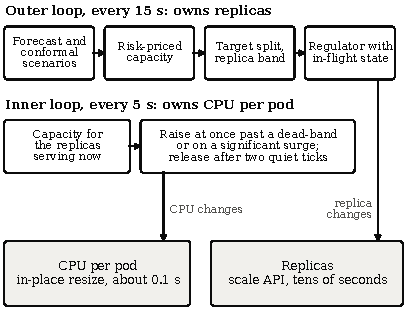
\includegraphics[width=0.62\textwidth]{fig_architecture.pdf}\\
\small Figure 1. The two loops. The outer loop (top) owns the number of pods; the inner
loop (middle) owns the CPU of each pod.
\end{center}

\newpage
%=====================================================================
\part*{Part 2 \quad How CHIMERA works and how it was tested}
\addcontentsline{toc}{part}{Part 2: How CHIMERA works and how it was tested}

\section{How CHIMERA works, step by step}

Every 15 seconds the \textbf{outer loop} runs steps 1--4. Every 5 seconds the
\textbf{inner loop} runs step 5.

\subsection*{Step 1: Forecast the traffic, with an honest range}
A machine-learning model (LightGBM quantile regression) predicts next minute's traffic as
a range (CQR, 90\,\% confidence). Because a learned model can be badly wrong on traffic it
has never seen, a second, simple margin is kept beside it: ``last value plus the size of
recent minute-to-minute jumps''. A drift detector (ADWIN) notices when the traffic pattern
has changed and makes the margin forget the old pattern.

\subsection*{Step 2: Decide how much total CPU is worth paying for (risk pricing)}
Instead of the usual fixed rule ``keep utilisation at 70\,\%'', CHIMERA asks: \emph{for
each extra core, how many slow requests does it prevent, and is that worth its price?}
It takes several possible futures (current traffic, current traffic plus each recent
jump, the forecast's upper bound), and picks the capacity $c$ that minimises
\[
\underbrace{\text{expected number of slow requests over those futures}}_{\text{bad for users}}
\;+\; \underbrace{\lambda \times c}_{\text{cost of CPU}} .
\]
The price $\lambda$ is set so that if the future were certain, the answer is simply
``demand divided by a target utilisation'' (CHIMERA's default setting is 0.46). When the
future is uncertain, it buys extra headroom only where the risk is real.

\subsection*{Step 3: Split the capacity into pods $\times$ CPU, and keep pods still}
Total capacity $c$ can be reached many ways: 2 pods of 2 cores, 4 pods of 1 core, and so
on. Adding a pod costs boot time (a pod that is starting is paid for but does no work).
So CHIMERA uses a \textbf{replica band}: as long as the current number of pods can carry
the needed capacity by resizing CPU alone (within 85\,\% of each pod's maximum and above
its minimum), it does \emph{not} change the number of pods. CPU per pod is sized for the
pods that are serving \emph{now}, so the fast actuator covers the gap while new pods boot,
and hands CPU back when they arrive.

\subsection*{Step 4: The regulator that remembers pods in flight}
The outer loop's decision is made by an LQR controller. Its ``state'' (what it looks at)
is:
\[
e = [\;\text{CPU per pod} - \text{target},\;\; \text{serving pods} - \text{target pods},\;\;
\text{pods ordered last step but not ready yet}\;] .
\]
The third number is the important one. Because the controller knows those pods are on
their way, it does not order them again. With a 20\,s boot time and a 15\,s loop, one
``in flight'' slot is enough. The LQR gain $K$ is computed once by solving the Riccati
equation, and the Riccati solution also proves the loop is stable (it gives a Lyapunov
function for free).

\subsection*{Step 5: The fast inner loop (every 5 seconds)}
Only this loop changes CPU:
\begin{itemize}
\item \textbf{Raise at once} if the CPU needed is more than 30\,\% above the current
allocation (the \emph{dead-band}, which stops tiny back-and-forth changes), or if a
statistical test shows a genuine surge in the last few seconds.
\item \textbf{Give CPU back} once the need has stayed 15\,\% below the allocation for two
checks in a row (10 seconds). Getting CPU back takes 0.1\,s, so there is no reason to hold
it ``just in case''.
\end{itemize}

\subsection*{A worked example}
\begin{enumerate}
\item Quiet traffic: 2 pods with 0.5 cores each. Everything is calm.
\item A surge starts. Within 5 seconds the inner loop sees it and raises each pod to
0.9 cores, in place, in 0.1\,s. No pod restarts. The users barely notice.
\item The surge keeps growing. Two pods at their maximum CPU are not enough, so the outer
loop orders 2 more pods and records ``2 in flight''.
\item 15 seconds later the new pods are not ready yet. A normal autoscaler might order 2
more. CHIMERA sees ``2 in flight'' and waits.
\item The new pods become ready. CPU per pod is now more than needed, so the inner loop
lowers it: the fast actuator hands the capacity back.
\item The surge ends. CPU drops within about 10 seconds; pods are removed later, more
carefully.
\end{enumerate}

\subsection*{What was removed, and why}
The original design (``v1'') also had a \emph{coupling penalty} (punishing the two
actuators for moving in opposite directions) and a \emph{Lyapunov safety filter} (checking
every action for stability). Tests showed both change \textbf{no decision at all}: once
each actuator has a single owner, opposite moves do not happen, and the LQR is already
proven stable. They were taken out of the final controller (v6). This is reported openly.

\section{The competitors (baselines)}

\begin{center}
\begin{tabular}{@{}p{3.2cm}p{11.8cm}@{}}
\toprule
\textbf{Baseline} & \textbf{What it does} \\
\midrule
HPA & Kubernetes standard. Adds/removes pods of fixed size (0.5 cores) to keep CPU near a target (70\,\%). Reactive. \\
VPA & Five fixed pods; changes their CPU size from usage. \\
HPA+VPA & Both standard tools running together on the same CPU signal. \\
AAPA & The paper this project started from (arXiv 2507.05653). Classifies traffic into four types (spike, periodic, ramp, stationary) and uses a tuned policy for each, with confidence. Pods only. \\
MagicScaler-style & Our implementation of the idea of MagicScaler (VLDB 2023): forecast with uncertainty, choose the number of pods trading cost against the risk of slow requests. Pods only. \\
KOSMOS & ICSOC 2021. Changes CPU every 5\,s with a PI controller on response time, and pods every 300\,s with rules. The closest existing system. Reimplemented from the paper. \\
\bottomrule
\end{tabular}
\end{center}

All controllers get the same limits (CPU per pod 0.5--4 cores, 2--30 pods) and start from
the same state.

\section{How it was tested}

\subsection{The simulator}
Running thousands of experiments on a real cluster is impossible, so most testing uses a
\textbf{simulator} (built on the open-source AAPA simulator, extended to two dimensions).
It models: requests arriving randomly, each needing on average 0.1\,s of CPU; the
slow-down when CPU gets busy ($\frac{1}{1-u}$); a new pod taking 20\,s to boot; an
in-place resize taking 0.1\,s; and an SLO of 0.5\,s. One run simulates 30 scored minutes of
a trace (after a 20-minute unscored warm-up, so nobody is judged on its cold start).

\subsection{The traffic (four sets of traces)}
\begin{center}
\begin{tabular}{@{}lp{8.6cm}l@{}}
\toprule
\textbf{Set} & \textbf{What} & \textbf{Used for} \\
\midrule
Dev & 5 Azure Functions traces (an earlier time window) and 4 synthetic shapes & designing \\
Held-out & the same 5 Azure traces (a later window) and 4 \emph{different} synthetic shapes (flash crowd, daily cycle, step down, on/off) & judging \\
Serverless & 10 real production functions from Huawei Cloud (2023, public, CC BY 4.0) & judging \\
Web & 10 windows from NASA (1995) and ClarkNet (1995) web-server logs & judging \\
\bottomrule
\end{tabular}
\end{center}
\textbf{The rule:} every design choice was made on the dev set only. The verdict comes from
data no design decision saw. The serverless and web traces were chosen by a fixed rule
written down \emph{before} any controller ran on them. This prevents ``tuning to the
test''.

\subsection{The fair comparison: at equal CPU}
Comparing each autoscaler at its default setting is misleading: one that spends more CPU
will naturally have fewer slow requests. So every autoscaler is run at several settings
(from generous to stingy), which gives a \textbf{cost--violation curve} (a ``frontier'')
for each. Then, for each trace, we ask: \emph{at exactly the CPU cost CHIMERA used, how
many slow requests would the other autoscaler have?} (read off its curve). If CHIMERA's
number is lower, CHIMERA wins that comparison.

\subsection{Statistics}
Each comparison is repeated with 5--10 seeds. A Wilcoxon signed-rank test checks whether
the differences are consistently in one direction (not luck), and a Holm correction
adjusts for testing several baselines at once. ``$p<0.001$'' means the result is very
unlikely to be chance.

\subsection{Scale of the experiments}
Held-out set: 3,870 main runs plus 4,095 sweep runs. Each external set: 900 + 3,150 runs.
Robustness: 8 scenarios $\times$ 2,205 runs. Plus ablations, tuning runs and the live
experiments: well over 30,000 simulated runs in total.

\newpage
%=====================================================================
\part*{Part 3 \quad Results}
\addcontentsline{toc}{part}{Part 3: Results}

\section{Where CHIMERA outperforms}

\subsection{At equal CPU, against everything}
\begin{center}
\begin{tabular}{@{}lrrrrrr@{}}
\toprule
 & \multicolumn{2}{c}{Held-out} & \multicolumn{2}{c}{Serverless (Huawei)} & \multicolumn{2}{c}{Web (NASA, ClarkNet)} \\
\cmidrule(lr){2-3}\cmidrule(lr){4-5}\cmidrule(l){6-7}
Baseline & traces won & gap & traces won & gap & traces won & gap \\
\midrule
AAPA & 9/9 & +3.30 & 10/10 & +2.02 & 10/10 & +2.00 \\
HPA & 9/9 & +6.19 & 10/10 & +3.99 & 10/10 & +4.53 \\
HPA+VPA & 9/9 & +5.16 & 10/10 & +2.72 & 10/10 & +3.89 \\
KOSMOS & 9/9 & +5.81 & 10/10 & +2.38 & 10/10 & +1.27 \\
MagicScaler-style & 8/9 & +5.87 & 10/10 & +4.37 & 10/10 & +4.66 \\
VPA & 6/6 & +6.00 & 9/9 & +1.77 & 10/10 & +2.20 \\
\bottomrule
\end{tabular}\\[3pt]
\small ``Gap'' = baseline's SLO violation rate minus CHIMERA's, in percentage points, at the same CPU
cost. All $p<0.001$.
\end{center}

\textbf{Headline:} 47 of 48 comparisons won on the held-out set, and \textbf{117 of 117} on
the twenty real traces never used in design.

\begin{center}
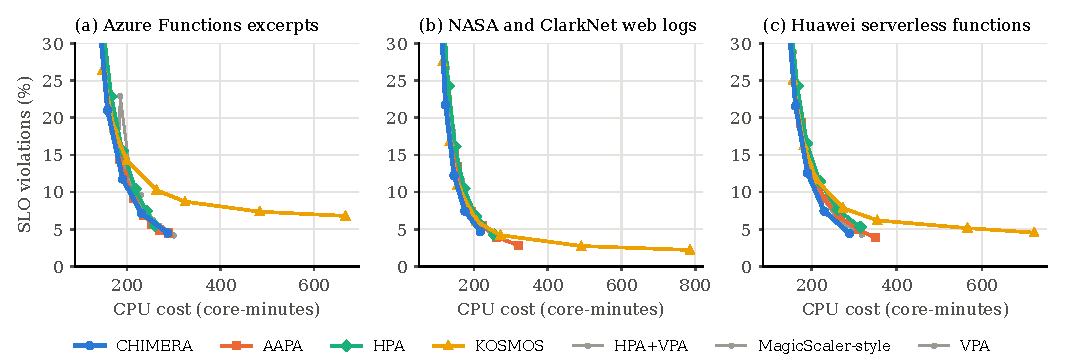
\includegraphics[width=\textwidth]{fig_frontiers.pdf}\\
\small Figure 2. Cost (x) against slow requests (y) for each autoscaler at several
settings. Down-left is better. CHIMERA's curve (blue) is the lowest.
\end{center}

\subsection{At default settings}
\begin{center}
\begin{tabular}{@{}lrrrr@{}}
\toprule
 & \multicolumn{2}{c}{Held-out, Azure traces} & \multicolumn{2}{c}{Serverless (Huawei)} \\
\cmidrule(lr){2-3}\cmidrule(l){4-5}
Autoscaler & SLO violations & CPU (core-min) & SLO violations & CPU (core-min) \\
\midrule
\textbf{CHIMERA} & \textbf{5.93\,\%} & 251.5 & \textbf{6.06\,\%} & 251 \\
AAPA & 6.92\,\% & 236.8 & 9.18\,\% & 230 \\
KOSMOS & 8.71\,\% & 326.7 & 6.16\,\% & 364 \\
HPA+VPA & 14.06\,\% & 194.8 & 14.75\,\% & 191 \\
HPA & 15.60\,\% & 190.8 & 16.47\,\% & 190 \\
MagicScaler-style & 16.78\,\% & 181.1 & 19.21\,\% & 179 \\
VPA & 19.40\,\% & 169.2 & 21.85\,\% & 169 \\
\bottomrule
\end{tabular}
\end{center}
p99 latency on the Azure traces: CHIMERA 0.82\,s, AAPA 0.91\,s, HPA 3.65\,s, KOSMOS
3.87\,s.

\subsection{It still holds when the simulator's rules change}
Because CHIMERA's risk pricing uses the same latency formula as the simulator, a fair
critic asks: ``Does it only win because it knows the simulator's rules?'' We re-ran the
held-out comparison with 8 different latency laws (different request-size distributions
and different slow-down formulas), without re-tuning CHIMERA.
\begin{itemize}
\item In 6 of 8 scenarios CHIMERA still wins every comparison (42/42).
\item With ``bimodal'' requests (10\,\% of requests are very slow), it wins 37--38 of 42
and loses narrowly to AAPA on four traces.
\item The risk-pricing part specifically is worth about 1 point when its formula matches,
and about 0 when it does not. The \emph{structure} (fast loop, single owner, replica band,
in-flight memory) carries the robust part of the win.
\end{itemize}

\begin{center}
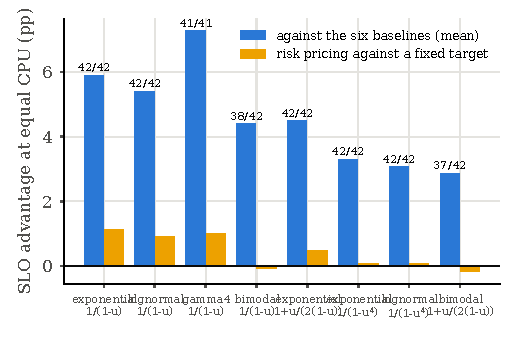
\includegraphics[width=0.6\textwidth]{fig_robustness.pdf}\\
\small Figure 3. Blue: advantage over the six baselines under each latency law. Orange:
what risk pricing alone adds.
\end{center}

\subsection{Which parts matter (ablation)}
\begin{center}
\begin{tabular}{@{}lrrrr@{}}
\toprule
Variant (held-out, Azure traces) & Violations & CPU & Resizes/run & Pod changes/run \\
\midrule
Full CHIMERA & 5.93\,\% & 251.5 & 32.5 & 0.5 \\
without fast release & 2.24\,\% & 480.1 & 1.0 & 0.5 \\
pods only (no CPU resizing) & 4.80\,\% & 271.7 & 12.0 & 12.0 \\
without the 5\,s inner loop & 4.92\,\% & 274.6 & 37.2 & 0.4 \\
without the 30\,\% dead-band & 4.96\,\% & 269.1 & 84.1 & 0.5 \\
without the replica band & 5.88\,\% & 256.2 & 43.3 & 8.6 \\
+ coupling penalty / + Lyapunov filter & 5.93\,\% & 251.5 & 32.5 & 0.5 \\
\bottomrule
\end{tabular}
\end{center}
How to read it: a row with fewer violations but much more CPU is just a more expensive
setting, not better. Without fast release CPU nearly \textbf{doubles}. Pods-only needs
8\,\% more CPU here (60\,\% more on the synthetic shapes) and changes pods 24 times as
often. The dead-band cuts resizes from 84 to 32 per run. The last row shows the two
removed parts change nothing.

\section{On a real cluster}

\subsection{It works on real Kubernetes}
The same controller runs as a Kubernetes \textbf{operator} (a program inside the cluster).
It reads CPU usage or request rate from \textbf{Prometheus} (a metrics system), resizes pods
through the \texttt{pods/resize} API, and changes pod counts through the scale API. It was
tested on a local cluster (\texttt{kind}, Kubernetes 1.33.1) and on an AWS server
(\texttt{t3.small}, k3s 1.33). Checks passed on both: real metrics, CPU raised in place
with \textbf{zero restarts}, pods added without flapping, CPU released after load, status
written back.

\subsection{Head-to-head with the Kubernetes HPA}
A load generator replayed a 24-minute trace (real Azure traffic, then a spike to five
times normal) against a real web service, measuring each request's latency. Both sides
could use at most 10 cores. Each autoscaler ran at three settings, three seeds each.

\begin{center}
\begin{tabular}{@{}lrr@{\qquad}lrr@{}}
\toprule
HPA target & Slow requests & CPU & CHIMERA setting & Slow requests & CPU \\
\midrule
70\,\% & 48.9\,\% & 85.3 & 0.46 (default) & 32.1\,\% & 80.9 \\
50\,\% & 23.5\,\% & 102.4 & 0.35 & 14.6\,\% & 93.6 \\
35\,\% & 16.3\,\% & 124.3 & 0.25 & \textbf{7.0\,\%} & 108.1 \\
\bottomrule
\end{tabular}\\[3pt]
\small Slow = over 0.3\,s. CPU in core-minutes. Mean of 3 seeds.
\end{center}

\begin{itemize}
\item \textbf{7 of the 9 HPA runs were beaten outright} by a CHIMERA run with the same
seed (less or equal CPU \emph{and} fewer slow requests). \textbf{No CHIMERA run was beaten
that way.}
\item At equal cost CHIMERA had fewer slow requests in 5 of 6 comparable runs (mean
11.9 points better).
\item CHIMERA at 0.25 had less than half the slow requests of the HPA's best setting, with
13\,\% less CPU.
\end{itemize}

\begin{center}
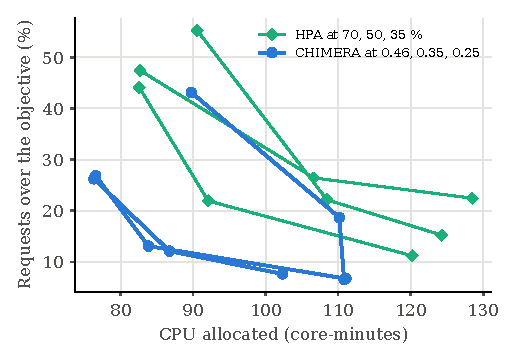
\includegraphics[width=0.55\textwidth]{fig_replay.pdf}\\
\small Figure 4. Real cluster. Each line is one seed. CHIMERA (blue) is below and left of
the HPA (green).
\end{center}

\begin{honest}[Be honest about the real-cluster result]
It is three seeds, one service, one trace, one laptop: \emph{indicative}, not
statistically proven. One CHIMERA run was repeated because the laptop interfered (the
service was slow even with far more CPU than needed); both attempts are kept and reported.
Every autoscaler had far more slow requests than in simulation, which shows the simulator
is kinder than reality.
\end{honest}

\section{Where CHIMERA does \emph{not} win}

\begin{honest}[Know these before the viva]
\begin{enumerate}
\item \textbf{KOSMOS at its default setting} has fewer slow requests than CHIMERA on three
of four trace groups (for example 4.22\,\% vs 6.18\,\% on the web traces), but uses
43--84\,\% more CPU and about ten times as many resizes. CHIMERA wins only once cost is
equal.
\item \textbf{The margins are modest}: about 2 points over AAPA and 1.3--2.4 over KOSMOS on
the real traces.
\item \textbf{One held-out loss}: the MagicScaler-style scaler on one flat, noisy Azure
trace, by 0.66 points.
\item \textbf{Bimodal requests}: loses narrowly to AAPA on 4 of 9 traces.
\item \textbf{Risk pricing} helps only when its latency formula is roughly right.
\item \textbf{More actions}: about 31 CPU resizes per half hour vs about 7 pod changes for
AAPA. Each resize is cheap, but the load on Kubernetes at very large scale was not
measured.
\item \textbf{The novelty is the combination}, not the individual ideas (see Section 11).
\end{enumerate}
\end{honest}

\section{The story of the project: versions, mistakes and fixes}

\subsection{Versions}
\begin{center}
\begin{tabular}{@{}lp{9.6cm}r@{}}
\toprule
Version & What changed & Azure SLO viol. \\
\midrule
v1 & first design: LQR + coupling penalty + Lyapunov filter & 11.82\,\% \\
v2 & fixed in-flight counting, vertical bridging, conformal margin & 7.06\,\% \\
v3 & added the 5\,s inner loop (cascade) & 7.35\,\% \\
v4 & inner loop owns CPU, replica band, drift reset & 7.39\,\% \\
v5 & risk-priced capacity & 6.13\,\% \\
v6 (final) & removed inert parts; 30\,\% dead-band halved resizes & 5.93\,\% \\
\bottomrule
\end{tabular}
\end{center}
(All re-measured on the same held-out data. v3 and v4 look slightly worse at default
settings because they spend less CPU; at equal CPU, v6 beats every earlier version: v1 by
about 7.9 points, v2 by 1.9, v3 by 1.4, v4 by 1.1 and v5 by 0.3.)

\subsection{Mistakes found and corrected (this is a strength, explain it as one)}
\begin{itemize}
\item \textbf{Simulator bugs that affected everyone:} the load sensor could not report more
than 6.7 requests per second; shared state leaked between runs. Fixed for all
controllers.
\item \textbf{Unfair baselines:} MagicScaler under-provisioned 3 times (wrong pod size);
HPA+VPA's VPA part never fired. Fixed before comparing.
\item \textbf{KOSMOS was mis-tuned.} Its settings were tuned before a simulator fix and made
it oscillate. Re-tuned on dev data, its violations fell from 19.8\,\% to 8.7\,\%. Our
claimed advantage over it fell from 19 points to about 6, and ``26 times better tail
latency'' became 4.7 times. We published the corrected numbers.
\item \textbf{An inflated claim:} ``19 times better p99 than AAPA'' was mostly AAPA
starting cold; with a warm-up it is 1.1 times.
\item \textbf{A discarded experiment:} the first web-trace run scaled traffic so high that
the pod-only baselines hit their 30-pod limit; CHIMERA's ``wins'' there were unfair. We
discarded it and re-ran with fair scaling.
\item \textbf{Real-cluster bugs the simulator could not show:} a pod that booted faster
than expected was counted twice and removed 15\,s after being added; four similar operator
problems followed. Each was fixed and has an automatic test.
\item \textbf{Fake references:} two papers in an early draft could not be found anywhere
and were removed.
\end{itemize}

\section{What is new, and what is not}
Honest positioning, after reading the closest papers:
\begin{itemize}
\item \textbf{Not new:} resizing in place before adding pods (Themis, 2024); optimising
pods and CPU together (Ship et al., IEEE CLOUD 2024); trading cost against risk
(MagicScaler, 2023); conformal prediction in an autoscaler (BACC, 2026).
\item \textbf{New in CHIMERA:} (1) one feedback controller that explicitly tracks pods
still booting, for the pair of a 0.1\,s and a 20\,s actuator; (2) handing CPU back as
pods arrive, plus a band in which pods do not move; (3) conformal ``possible futures'' used
to price risk, in a rule that reduces to an ordinary target when the future is certain;
(4) an evaluation that separates design data from judging data, compares at equal cost,
and reports what did not work.
\end{itemize}

\section{Limitations}
\begin{enumerate}
\item Most numbers come from simulation; the real-cluster study is small.
\item Twenty real traces, 100 minutes each, from three sources.
\item The held-out set was used twice (v5, then v6); the v6 change was chosen on dev data
by a rule written beforehand.
\item KOSMOS and MagicScaler are our implementations, not the authors' code.
\item The simulator's boot time and resize time are constants; reality varies.
\item Only CPU is scaled, not memory.
\item The CPU cost of a request must be given to the operator when it uses request rate.
\end{enumerate}

\newpage
%=====================================================================
\part*{Part 4 \quad Viva preparation}
\addcontentsline{toc}{part}{Part 4: Viva preparation}

\section{Project map and how to run it}

\subsection{Important files}
\begin{center}
\begin{tabular}{@{}lp{10.2cm}@{}}
\toprule
\texttt{src/core/chimera\_controller.py} & the LQR controller (Riccati, in-flight state, lean path) \\
\texttt{src/core/chimera\_simulator.py} & the 2-D cluster simulator and CHIMERA's loops \\
\texttt{src/scripts/run\_full\_evaluation.py} & runs every controller on every trace and seed \\
\texttt{k8s/operator\_core.py}, \texttt{k8s/manager.py} & the real Kubernetes operator \\
\texttt{k8s/replay/} & the real-cluster head-to-head experiment \\
\texttt{tests/} & 18 simulator tests, 32 operator tests \\
\texttt{results/REPORT\_v6.md} & held-out results \\
\texttt{results/REPORT\_hw.md}, \texttt{REPORT\_ext.md} & serverless and web results \\
\texttt{results/replay3/REPLAY\_REPORT.md} & real-cluster results \\
\texttt{paper/chimera.pdf} & the conference paper \\
\texttt{IMPROVEMENT\_AUDIT.md} & every check, mistake and fix \\
\texttt{DEMO.md}, \texttt{demo/RUN\_DEMO.cmd} & the lab demo \\
\bottomrule
\end{tabular}
\end{center}
Code: \url{https://github.com/adithyan-css/CHIMERA_OS}

\subsection{Live demo in two steps}
\begin{enumerate}
\item Start Docker Desktop and wait for ``Engine running''.
\item Double-click \texttt{demo\textbackslash RUN\_DEMO.cmd} and follow the prompts. It
checks the cluster, runs the simulation comparison, opens two windows (operator decisions,
pods and CPU), adds load (watch the CPU of the same pods rise with zero restarts), removes
it (watch the CPU come back), and opens the paper.
\end{enumerate}

\section{Viva questions and answers}

\subsection*{The basics}
\Q{What is CHIMERA in one sentence?}
\A A Kubernetes autoscaler that controls both the number of pods and the CPU of each pod
with one coordinated decision, using the fast actuator (in-place resize) first and
remembering pods that are still starting.

\Q{What problem does it solve?}
\A Keeping requests fast at the lowest CPU cost when traffic changes, now that CPU can be
resized in 0.1\,s while new pods still take tens of seconds.

\Q{What is horizontal vs vertical scaling?}
\A Horizontal: more pods. Vertical: more CPU per pod. Horizontal is slow (boot time),
vertical is fast since in-place resize.

\Q{What is in-place pod resize, and why does it matter?}
\A Kubernetes feature (KEP-1287, on by default from 1.33) that changes a running pod's CPU
without restarting it. Without it, vertical scaling would need a restart and could not be
used for fast reactions; with it removed, CHIMERA's violations on the synthetic traces rise
from 5.63\,\% to 7.91\,\%.

\Q{What is an SLO and what is an SLO violation?}
\A A latency promise, here 0.5\,s per request in simulation (0.3\,s on the real service).
A violation is a request slower than that. We report the percentage of such requests.

\Q{Why not just give the application lots of CPU?}
\A Cost. Every allocated core is paid for. The goal is the best latency for a given cost,
which is why we compare at equal CPU.

\Q{What is a core-minute?}
\A One core allocated for one minute. Our cost measure.

\subsection*{How it works}
\Q{What are the two loops?}
\A Outer, every 15\,s: decides total capacity and the number of pods (LQR). Inner, every
5\,s: changes CPU per pod only (raise past a 30\,\% dead-band or on a surge; release after
two quiet checks).

\Q{Why two loops at different speeds?}
\A Each actuator gets a loop matching its speed and a single owner, so they never fight.
The ablation shows CPU nearly doubles without fast release, and resizes rise from 32 to 80
if both loops can change CPU.

\Q{What is LQR and why use it?}
\A Linear-quadratic regulator: an optimal feedback rule $u=-Ke$ balancing tracking error
against action size. It gives a principled joint decision and, through the Riccati
solution, a stability proof.

\Q{What is the ``in-flight'' state?}
\A The pods ordered last step that are not ready yet. Including them in the state stops
the controller ordering the same capacity twice. On the real cluster we reconcile it with
what Kubernetes reports (desired minus ready pods).

\Q{Why one in-flight slot?}
\A Boot time 20\,s, loop 15\,s: an order placed now is ready before the step after next,
so it is pending for exactly one step.

\Q{How do you prove stability?}
\A The Riccati solution $P$ is positive definite and $V=e^\top P e$ decreases under
$u=-Ke$, so $V$ is a Lyapunov function. That is why the separate Lyapunov filter never
acted and was removed.

\Q{What is risk-priced capacity?}
\A Choose total cores minimising expected slow requests over several plausible futures
plus a price per core. With a certain future it reduces to demand / target utilisation.

\Q{What is conformal prediction and why use it?}
\A A method that makes a forecaster's uncertainty range honest: it uses recent errors to
size the range so it covers the truth about 90\,\% of the time, without assuming a
distribution. We use it to build the possible futures.

\Q{What is the replica band?}
\A A range of pod counts within which the needed capacity can be reached by resizing CPU
alone. Inside it, pods are not added or removed, because each new pod wastes its boot time.
It cuts pod changes from 8.6 to 0.5 per run.

\Q{What is the dead-band and why 30\,\%?}
\A CPU is raised only if the need exceeds the allocation by more than 30\,\%. It stops tiny
back-and-forth resizes. 30\,\% was the widest value that did not hurt efficiency on the dev
data; it halved resizes (62 to 31 per run).

\Q{What is ADWIN?}
\A A drift detector: it notices when the traffic pattern changes, so the safety margin
forgets the old pattern.

\Q{Why did you remove the coupling penalty and the Lyapunov filter?}
\A Tests showed they changed no decision in any of 90 runs. Single ownership prevents
opposite moves, and the LQR is already stable. Removing them changed no result.

\subsection*{Testing}
\Q{Why a simulator?}
\A Tens of thousands of controlled, repeatable experiments with identical traffic for
every controller. A real cluster cannot do that in reasonable time. We then checked on a
real cluster.

\Q{How do you avoid tuning to the test data?}
\A All choices on a dev split; verdict on held-out data, plus twenty real traces chosen by
a rule written before any run.

\Q{What does ``at equal CPU'' mean?}
\A Each controller is run at several settings to get a cost--violation curve; we read each
baseline's violation rate at exactly CHIMERA's CPU cost. Otherwise a controller could look
better just by spending more.

\Q{What statistical test did you use?}
\A Wilcoxon signed-rank on paired gaps (same trace, same seed), Holm-corrected for multiple
baselines. All main comparisons $p<0.001$.

\Q{Why a 20-minute warm-up?}
\A So no controller is judged on its cold start. Without it, AAPA looked 19 times worse in
p99 than it really is.

\Q{What are the traces?}
\A Five Azure Functions excerpts, ten Huawei Cloud serverless functions (2023), ten NASA
and ClarkNet web-log windows (1995), plus synthetic shapes (flash crowd, daily cycle, step
down, on/off).

\subsection*{Results}
\Q{Does it outperform the others?}
\A At equal CPU, yes: 47 of 48 comparisons on the held-out set and 117 of 117 on the twenty
real traces, all significant. On a real cluster, 7 of 9 HPA runs were beaten outright and
no CHIMERA run was.

\Q{By how much?}
\A Modestly: about 2 percentage points fewer slow requests than AAPA at equal CPU on the
real traces, 1.3--2.4 than KOSMOS, 4--5 than HPA.

\Q{Which baseline is strongest?}
\A KOSMOS, after re-tuning. At its default setting it matches or beats CHIMERA's violation
rate on three of four trace groups but spends 43--84\,\% more CPU.

\Q{Where does CHIMERA lose?}
\A One held-out trace vs the MagicScaler-style scaler (0.66 points); four traces vs AAPA
when requests are bimodal; KOSMOS at default settings if you ignore cost.

\Q{Which part gives the most benefit?}
\A Fast release of CPU, then joint control (using CPU resizing at all), then single
ownership and the dead-band. Risk pricing adds about one point and depends on its model.

\Q{How did it do on the real cluster?}
\A Against the Kubernetes HPA with three settings each and three seeds: CHIMERA at 0.25
had 7.0\,\% slow requests at 108 core-minutes vs the HPA's best 16.3\,\% at 124; 7 of 9 HPA
runs beaten outright, none the other way. Zero container restarts in all runs.

\Q{Why were violation rates so high on the real cluster?}
\A A 61\,ms request on a pod limited to half a core exceeds one CPU-quota period, so the
real service queues much more than the simulator's formula assumes. It applies to every
autoscaler equally; it shows the simulator is optimistic.

\subsection*{Critical questions}
\Q{Isn't this only simulation?}
\A Most numbers are, but the operator runs on real Kubernetes (local and AWS), and a
real-cluster comparison with measured latency points the same way. That study is small and
we say so.

\Q{Did you tune CHIMERA more than the baselines?}
\A No more: KOSMOS was re-tuned on dev data like CHIMERA, baselines had bugs fixed before
comparison, and every controller is compared along its whole cost curve.

\Q{Your risk model matches the simulator. Isn't that cheating?}
\A We tested exactly that: 8 other latency laws without re-tuning. The win over baselines
survives; only the risk-pricing part's small gain disappears. We report this.

\Q{What is genuinely new?}
\A The combination: a feedback controller tracking pods in flight for a fast/slow actuator
pair, handing CPU back as pods arrive, a replica band, and conformal futures for risk
pricing, plus a careful evaluation. The individual ideas exist in Themis, Ship et al.,
MagicScaler and BACC.

\Q{Why so many CPU resizes?}
\A About 31 per half hour after the dead-band (down from 62). Resizes are cheap (0.1\,s, no
restart). KOSMOS makes about 250. Fleet-scale API load is untested.

\Q{What would you do next?}
\A A larger real-cluster study (several nodes, a multi-service app, more seeds, real AAPA
and KOSMOS operators); learn the latency curve from measurements; scale memory too.

\Q{Why is it called CHIMERA?}
\A A chimera combines parts of different creatures; the controller combines horizontal and
vertical scaling in one body.

\Q{What tools and languages?}
\A Python (NumPy, SciPy, LightGBM, SimPy, pandas), Kubernetes 1.33 (kind locally, k3s on
AWS EC2), Prometheus, Docker, LaTeX for the paper.

\Q{How long does one control step take?}
\A Well under a millisecond (about 0.3--0.5\,ms on a laptop), against a 5--15\,s loop.

\Q{How do you know the operator is correct?}
\A 32 automatic tests (including regression tests for each live bug), five live checks
passing on two clusters, and the head-to-head replay.

\section{Glossary}
\begin{longtable}{@{}p{3.6cm}p{11.4cm}@{}}
\toprule
\textbf{Term} & \textbf{Meaning} \\
\midrule
\endhead
Ablation & Removing one part to measure its effect. \\
ADWIN & Adaptive windowing: detects a change in a data stream. \\
Baseline & Existing method compared against. \\
Cascade & Two nested control loops: a fast inner one and a slower outer one. \\
Cluster & A group of machines run together by Kubernetes. \\
Conformal prediction & Distribution-free way to make prediction intervals with guaranteed coverage. \\
Container & A packaged program that runs the same way anywhere. \\
Core-minute & One CPU core allocated for one minute; cost unit. \\
CQR & Conformalized quantile regression. \\
Dead-band & A minimum change below which no action is taken. \\
Dev / held-out split & Data for designing vs data for judging. \\
Equal-CPU comparison & Comparing violation rates at the same CPU cost. \\
Frontier & Curve of cost vs violations as a controller's setting changes. \\
HPA / VPA & Kubernetes horizontal / vertical pod autoscalers. \\
In-flight pods & Pods ordered but not yet ready. \\
In-place resize & Changing a running pod's CPU without restart (KEP-1287). \\
kind, k3s & Small Kubernetes distributions (local in Docker; lightweight server). \\
LQR & Linear-quadratic regulator: optimal linear feedback control. \\
Lyapunov function & An ``energy'' that always decreases in a stable system. \\
Operator & A program inside Kubernetes that manages something automatically. \\
p99 & 99th-percentile latency. \\
Pod / replica & One running copy of the application / an additional copy. \\
Prometheus & Monitoring system that collects metrics. \\
Replica band & Range of pod counts in which CHIMERA keeps the count fixed. \\
Riccati equation & The equation whose solution gives the LQR gain and stability proof. \\
Seed & Starting value for random choices; same seed, same traffic. \\
SLO & Service level objective: the latency target. \\
Trace & A recording of real traffic over time. \\
Utilisation & Demand divided by capacity. \\
Wilcoxon test & Statistical test for consistent paired differences. \\
\bottomrule
\end{longtable}

\section{One page of numbers to remember}
\begin{viva}[Memorise this]
\begin{itemize}
\item Fast actuator: in-place resize, \textbf{0.1\,s}. Slow actuator: new pod, \textbf{20\,s}
boot (simulator).
\item Loops: outer \textbf{15\,s} (pods), inner \textbf{5\,s} (CPU). Dead-band
\textbf{30\,\%}; release after \textbf{2} checks \textbf{15\,\%} below. Default setting
\textbf{0.46}.
\item SLO: \textbf{0.5\,s} (simulator), \textbf{0.3\,s} (real service, 61\,ms per request).
\item Held-out: \textbf{47/48} wins at equal CPU. Real traces never used in design:
\textbf{117/117} (57 serverless + 60 web). All $p<0.001$.
\item Advantage at equal CPU on real traces: about \textbf{+2.0} points over AAPA,
\textbf{+1.3 to +2.4} over KOSMOS.
\item Defaults, Azure held-out: CHIMERA \textbf{5.93\,\%}, AAPA 6.92\,\%, HPA 15.60\,\%.
\item Robustness: wins all comparisons in \textbf{6 of 8} latency laws.
\item Ablation: no fast release $\Rightarrow$ CPU \textbf{$\times$1.9}; replica band cuts pod
changes \textbf{8.6 $\to$ 0.5}; dead-band cuts resizes \textbf{84 $\to$ 32}.
\item Resizes per half hour: \textbf{about 31} (v5: 62; KOSMOS: about 250).
\item Real cluster vs HPA: \textbf{7 of 9} HPA runs beaten outright, \textbf{0} CHIMERA
runs beaten; CHIMERA 0.25: \textbf{7.0\,\%} at 108 core-min vs HPA best 16.3\,\% at 124.
\item KOSMOS re-tune: 19.8\,\% $\to$ 8.7\,\% violations; our advantage 19 $\to$ 6 points.
\item Tests: \textbf{18} simulator + \textbf{32} operator. Control step: \textbf{under 1\,ms}.
\item Versions: v1 11.82\,\% $\to$ v6 5.93\,\% (Azure held-out).
\end{itemize}
\end{viva}

\end{document}
